\section{Drehstrom- Synchronmaschinen(DSM)}
    \subsection{Aufbau der DSM}
        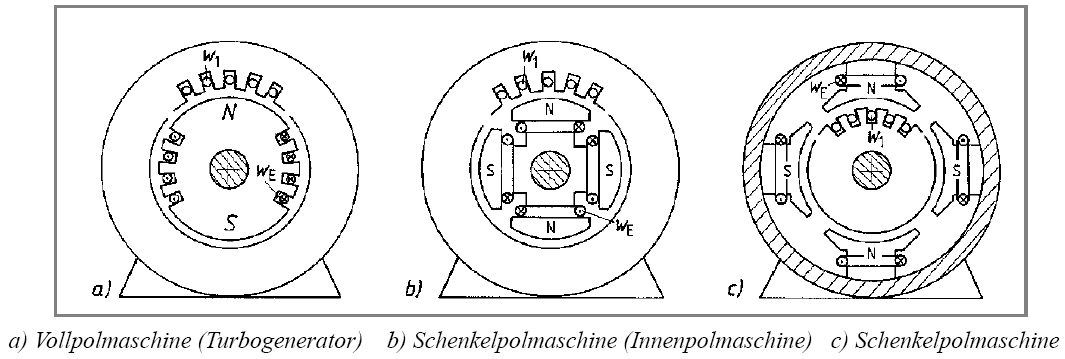
\includegraphics[width=12cm]{./images/Aufbau_DSM.png}\\
        \begin{tabular}{ p{1cm} p{4cm} p{10cm}}
            - &
            Innenpolmaschine: &
            Der Läufer ist ein Dauermagnet, oder wird mit Gleichstrom und über Schleifer zu einem solchem gemacht. Dieser läuft mit dem aussen anliegendem Drehfeld mit \\
            - &
            Aussenpolmaschine: &
            Der Läufer erzeugt ein Drehfeld, welches sich immer am konstanten Statorfeld ausrichtet. Worauf sich des Läufer dreht \\
            - &
            Turbomaschine: &
            Die Schleiferlose Variante. Mit Hilfe eines Hilfsgenerator auf der gleichen Welle wird ein Drehstrom erzeugt, welcher auf dem Läufer selbst gleichgerichtet wird. Damit wird dan ein konstantes Magnetfeld (Dauermagnet) erzeugt (wie die Innenpolmaschine) \\
        \end{tabular}

    \subsection{Ersatzschaltbild}
        \begin{minipage}{11cm}
            \abb{images/Ersatz_DSM.png}{8cm}{Ersatzschaltung DSM}    
            Es gibt 2 Unterteilungen:\\
            \begin{tabular}{p{1cm} p{9cm}}
                - &
                Wirkleistung: Gibt die DSM leistung ab oder nimmt sie auf. Zu erkennen ist das am Phasenwinkel zwischen $U_{KL}$ und $U_P$. Ist $U_P$ voreilend, so ist es ein \textbf{Generator}, anderseits ein \textbf{Motor}. \\
                - &
                Blindleistung: Blindleistung Auf- oder Abgabe. Bei \textbf{Übererregung} oder auch \textbf{kapazitiven Betrieb} gibt der DSM Blindleistung ab. Bei \textbf{Untererregung} oder auch \textbf{induktiven Betrieb} nimmt er auf. \\
            \end{tabular}
        \end{minipage}
        \begin{minipage}{8cm}
            \abb{images/Zeigerdiagram.png}{6cm}{Betriebszustände einer DSM}
        \end{minipage}\\

    \subsection{Betriebsverhalten}
        \begin{tabular}{l l l l}
            Leerlauf &
            \begin{minipage}{5cm}
                \abb{images/Leerlaufkennlinie.png}{4cm}{Im Betriebspunkt liniarisierte Leerlaufgerade}
            \end{minipage} &
            $I_E = \frac{U_P \cdot \sqrt{3} \cdot I_{E0N}}{U_N}$ &
            \begin{minipage}{9cm}
                Die Formel ist für die liniarisierte Gerade \\
                $I_E: $Erregerstrom \\
                $U_P: $verkettete Nennspannung des DS- Netzes\\
                $I_{E0N}:$Leerlauferregerstrom für Nennspannung
            \end{minipage} \\
        \end{tabular} \\
        \\
        \begin{tabular}{l l l l}
            Kurzschluss &
            \begin{minipage}{5cm}
                \abb{images/Kurzschlussgerade.png}{4cm}{Kurzschlussgerade}
            \end{minipage} &
            $X_d=\frac{U_P}{I_{K0}}$ &
            \begin{minipage}{9cm}
                Gilt unter Vernachlässigung des Wicklungswiderstand \\
                Die Kurzschlussgerade ist liniar
            \end{minipage} \\
        \end{tabular}

    \subsubsection{Inselbetrieb}
        \begin{minipage}{10cm}
            \abb{images/Belastungskennlinie_DSM.png}{9cm}{Belastungskennlinie bei konst. Erregerstrom}
        \end{minipage}
        \begin{minipage}{6cm}
            \abb{images/Regulierungslinie_DSM.png}{6cm}{Regulierungskennlinie für konst. $U_{Kl}$}
        \end{minipage} \\
        Die Klemmenspannung nimmt bei kapazitiven Lasten zu, bei induktiven stark ab. Für eine konstante $U_{Kl}$ muss der Erregerstrom wie die Regulierungskennlinie angepasst werden.

    \subsubsection{Netzbetrieb}
        Im Netzbetrieb wird die Frequenz, Klemmenspannung, Umlaufsinn und Phasenlage vom Netz vorgegeben. Das heisst bevor man mit einer DSM ans Netz will, muss man sie so synchronisieren, dass alle jene Parameter mit dem Netz überreinstimmen. Sind die Maschine und Netz synchronisiert und zusammengeschaltet, kann mit Hilfe von $I_E$ und der mechanischen Leistung der Blindstromanteil eingestellt werden: \\
        \begin{minipage}{8.2cm}
            \abb{images/Ortskurve_DSM.png}{8cm}{Ortskurve einer DSM im starren Netz}
        \end{minipage}
        \begin{minipage}{9.7cm}
            \begin{itemize}
                \item Da $U_{Kl} = U_1$ konstant ist, ist der Ursprung des Zeigers $\frac{j \cdot U_p}{X_d}$ immer am gleichen Ort. 
                \item Mit dem Erregerstrom kann man die Länge des Zeigers $\frac{j \cdot U_p}{X_d}$ einstellen.
                \item Die mechanische Leistung ist proportional zum Abstand der Zeigerspitze zur Imaginärachse.
                \item Die Blindleistung ist proportional zum Abstand  der Zeigerspitze zur Reelenachse.
                \item Ist nun die mechanische Leistung konstant und man ändert den Erregerstrom, so wandert die Zeiger auf einer Linie parallel zur Imag-Achse hin und her.
                \item Überschreitet der Zeiger die Stabilitätslinie, schlipft der Läufer durchund es gibt grosse Lärm- und Wärmeentwicklung, da die mechanische Leistung zu gross wird für den Erregerstrom.
                \item Bleibt der Erregerstrom konstant und die mechanische Leistung ändert sich, so wandert der Zeiger auf dem Kreis um (0,$\frac{U_Kl}{j \cdot X_d}$). Jedoch wiederum nur bis zur Stabilitätsgrenze, da dort die Wirkleistung für diesen Erregerstrom maximal ist.
            \end{itemize}
        \end{minipage}
        \\ \\ \\
        $$ U_P = \sqrt{\frac{U^2_{Netz}}{3} + X_d^2 \cdot I^2 + 2 \cdot \frac{U_{Netz}}{\sqrt{3}}\cdot X_d \cdot I \cdot \sin(\varphi)} $$
        \newpage